\documentclass[../main.tex]{subfiles}
\graphicspath{{\subfix{../images/}}}

\begin{document}
% Identify here the order in which you plan to implement the subcomponents of your system and the order in which you plan to integrate such subcomponents and test the integration.
\\
\noindent
This section will be describe how the various components of the system will be implemented, integrated together and tested. 
The implementation, integration and test plan will follow a bottom-up approach, applied to the entire system, including both Server and Client side. \\
\\
Assuming that the external services are reliable, it is not required to do unit testing on them. 


\subsection{Development Process}
Integration and testing will be done incrementally since it facilitates bug tracking. 
Each component should be checked under unit testing, and this is done before, during and after integration of a new module into the main software package. This involves testing of each individual code module. 
\\
\\
The whole system will be implemented, tested and integrated using a bottom-up approach. The latest emphasizes coding and early testing, which can begin as soon as the first module has been specified. In this way, the system could be completed incrementally and could be tested in parallel to its implementation. The available elements are used in the construction of new and more powerful elements at every stage. 
\\
\\
The dependencies between components are described in the diagram below: 


\begin{figure}[H]
\centering
    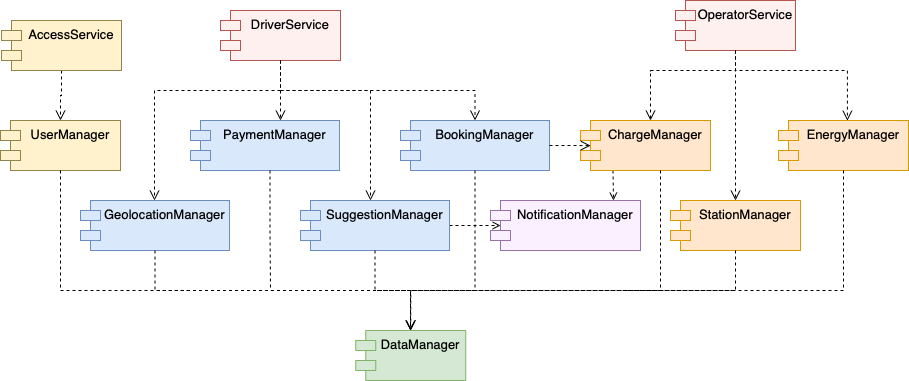
\includegraphics[width=1.05\textwidth]{images/DependencyDiagram.png}
    \caption{Dependency Diagram}
    \label{fig:deploymentDiagram}
\end{figure}

\subsection{Implementation Plan}
The implementation of the components of the Application Server is the follow: 
\begin{enumerate}
    \item \textbf{DataManager,NotificationManager} \\
    The first component that need to be implemented will be DataManager. We can clearly see on the component diagram that a lot of components of the server side relies on it for the communication with Database. Since NotificationManager does not depend on any component, it can be implemented in parallel with DataManager.
    
    \item \textbf{GeolocationManager, SuggestionManager, PaymentManager, BookingManager, ChargeManager, StationManager, EnergyManager, UserManager}\\
    These are the components of eMSP and others of the CPMS. Most of them can be implemented in parallel since they are independent to each other. They are dependent just on DataManager, which has been implemented before, and/or External APIs, which are ready to be used. \\
    The only problem we have is that BookingManager which is dependent on ChargeManager. This can be solved by implementing the main functionalities in ChargeManager which are required by BookingManager, so that the implementation of the latest can be started as soon as possible.

    \item \textbf{AccessService, DriverService, OperatorService}\\
    These components' functionalities heavily depend on the previous mentioned components, so that they must wait for those to be completed. However, these components are independent to each other so that they can be implemented in parallel.
    %\item \textbf{ClientApp, NotificationManager}\\
    %After the completion of all the previous components, we can finally complete with the implementation of ClientApp component, which is highly dependent on other components, and complete  the last part of the NotificationManager component which is dependent on ClientApp component. 
\end{enumerate}

\subsection{Integration Sequence}

In this section, the integration plan of the e-Mall system will be explained. Each component after its development will go under Unit Testing. After that integration testing process will start soon. The model will be integrated into the models of low level in order to test the behaviour of developed subsystem, in order to solve as many inconsistencies as possible.
\\
\\
In the diagram below, it’s shown then integration process at various levels of dependency. Note that Bottom-up strategy is used for those components which do not interact with external systems, while top-down strategy is used for the components which need to acquire information from external systems. 

\begin{figure}[H]
    \centering
    \begin{minipage}[b]{\textwidth}
        \centering
        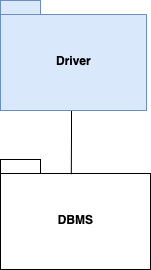
\includegraphics[width=30mm]{ImplementationDiagram/1.png}
        \caption{Initial state before integration}
        \label{fig:impdiag}
    \end{minipage}
\end{figure}

\begin{figure}[H]
    \centering
    \begin{minipage}[b]{\textwidth}
    \centering
    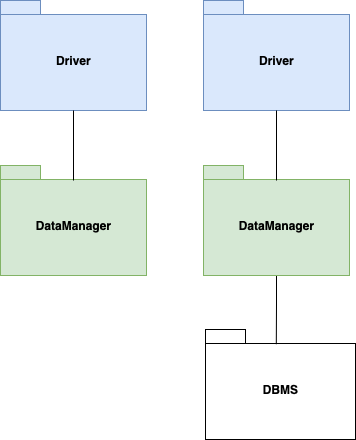
\includegraphics[width=30mm]{ImplementationDiagram/2.png}
    \caption{Integration of DataManager and NotificationManager}
    \label{fig:impdiag}
    \end{minipage}
\end{figure}

\begin{figure}[H]
    \centering
    \begin{minipage}[b]{\textwidth}
        \centering
        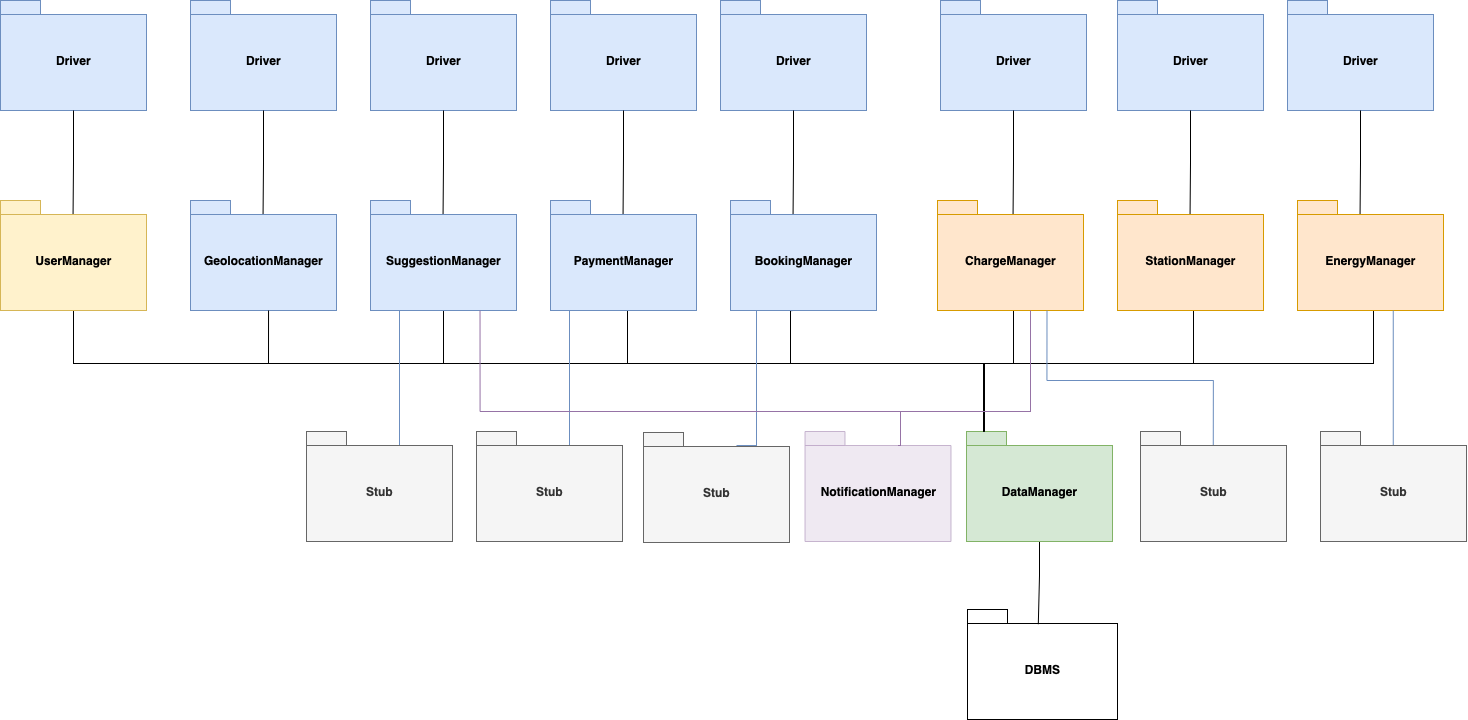
\includegraphics[width=1.05\textwidth]{ImplementationDiagram/3.png}
        \caption{Integration of GeolocationManager / SuggestionManager / PaymentManager / BookingManager / StationManager / ChargeManager / EnergyManager / UserManager}
        \label{fig:impdiag}
    \end{minipage}
\end{figure}


\begin{figure}[H]
    \centering
    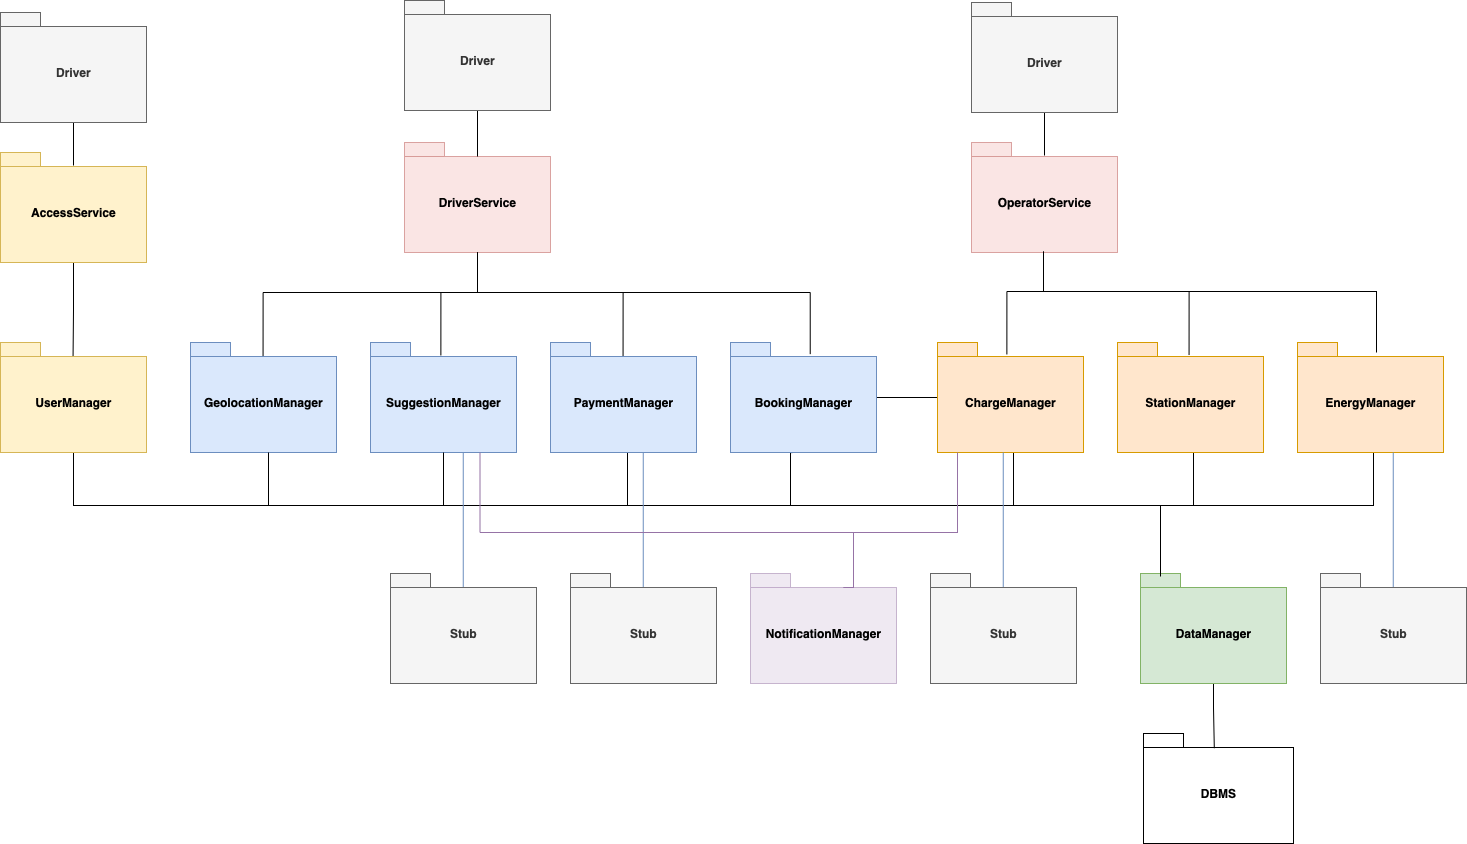
\includegraphics[width=1.05\textwidth]{ImplementationDiagram/4.png}
    \caption{Integration of AccessService/ DriverService/ OperatorService}
    \label{fig:impdiag}
\end{figure}

\begin{figure}[H]
    \centering
    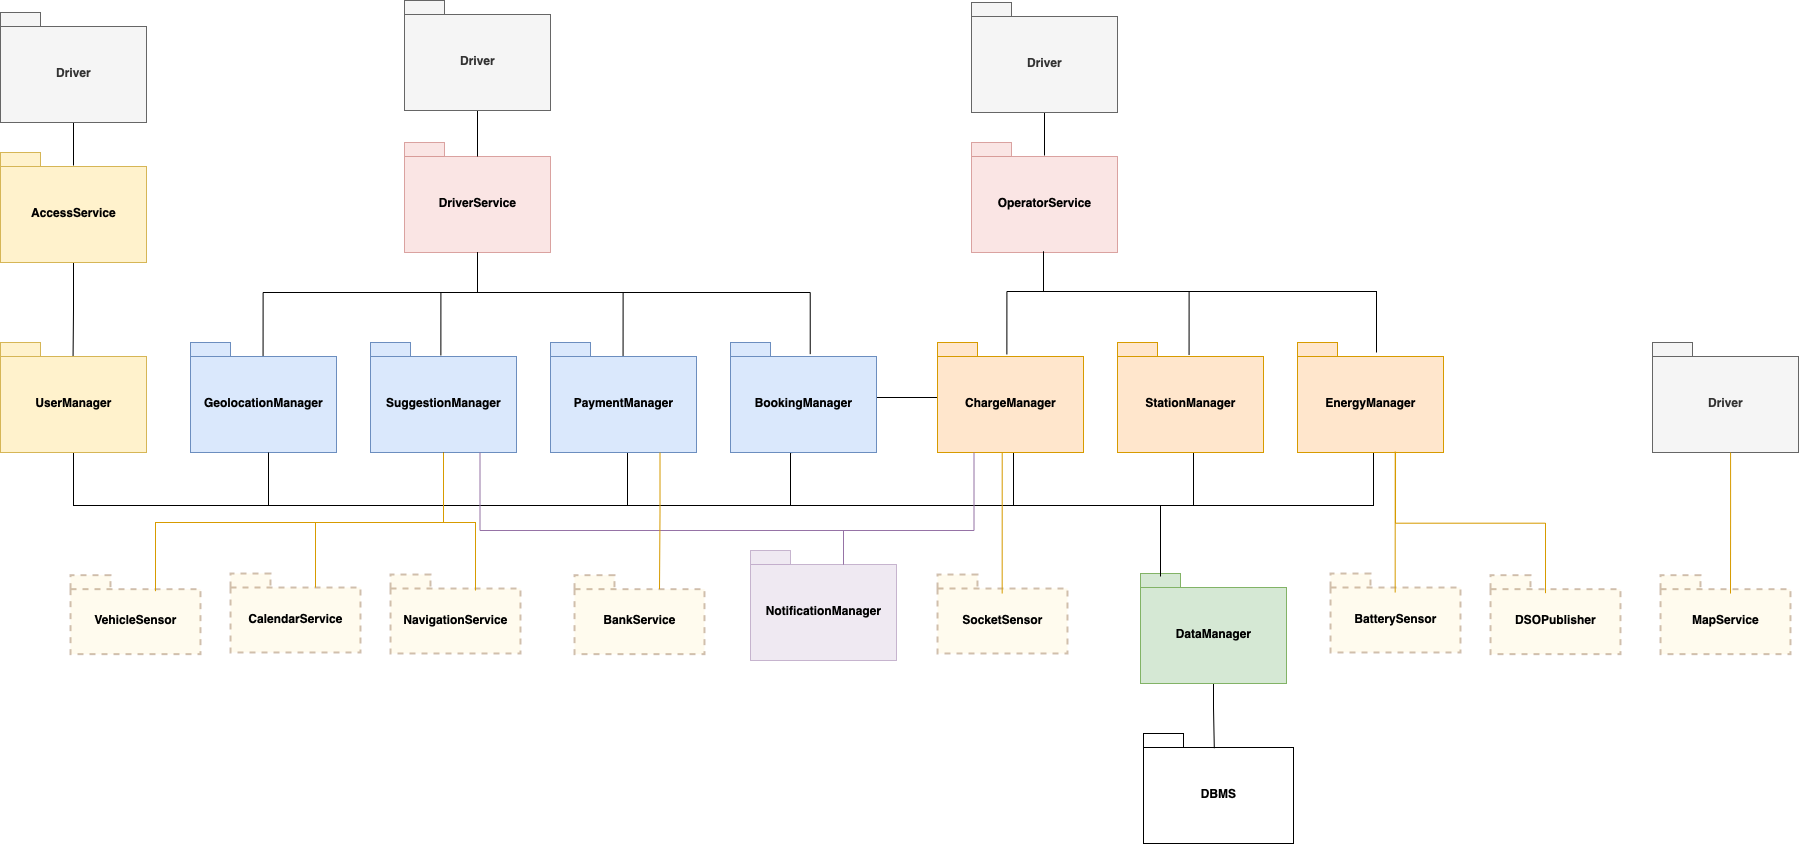
\includegraphics[width=1.05\textwidth]{ImplementationDiagram/5.png}
    \caption{Integration of external services: CalendarService/ NavigationService/ VehicleSensor/ BankService/ SocketSensor/ BatterySensor/ DSOPublisher/ MapService}
    \label{fig:impdiag}
\end{figure}

\begin{figure}[H]
    \centering
    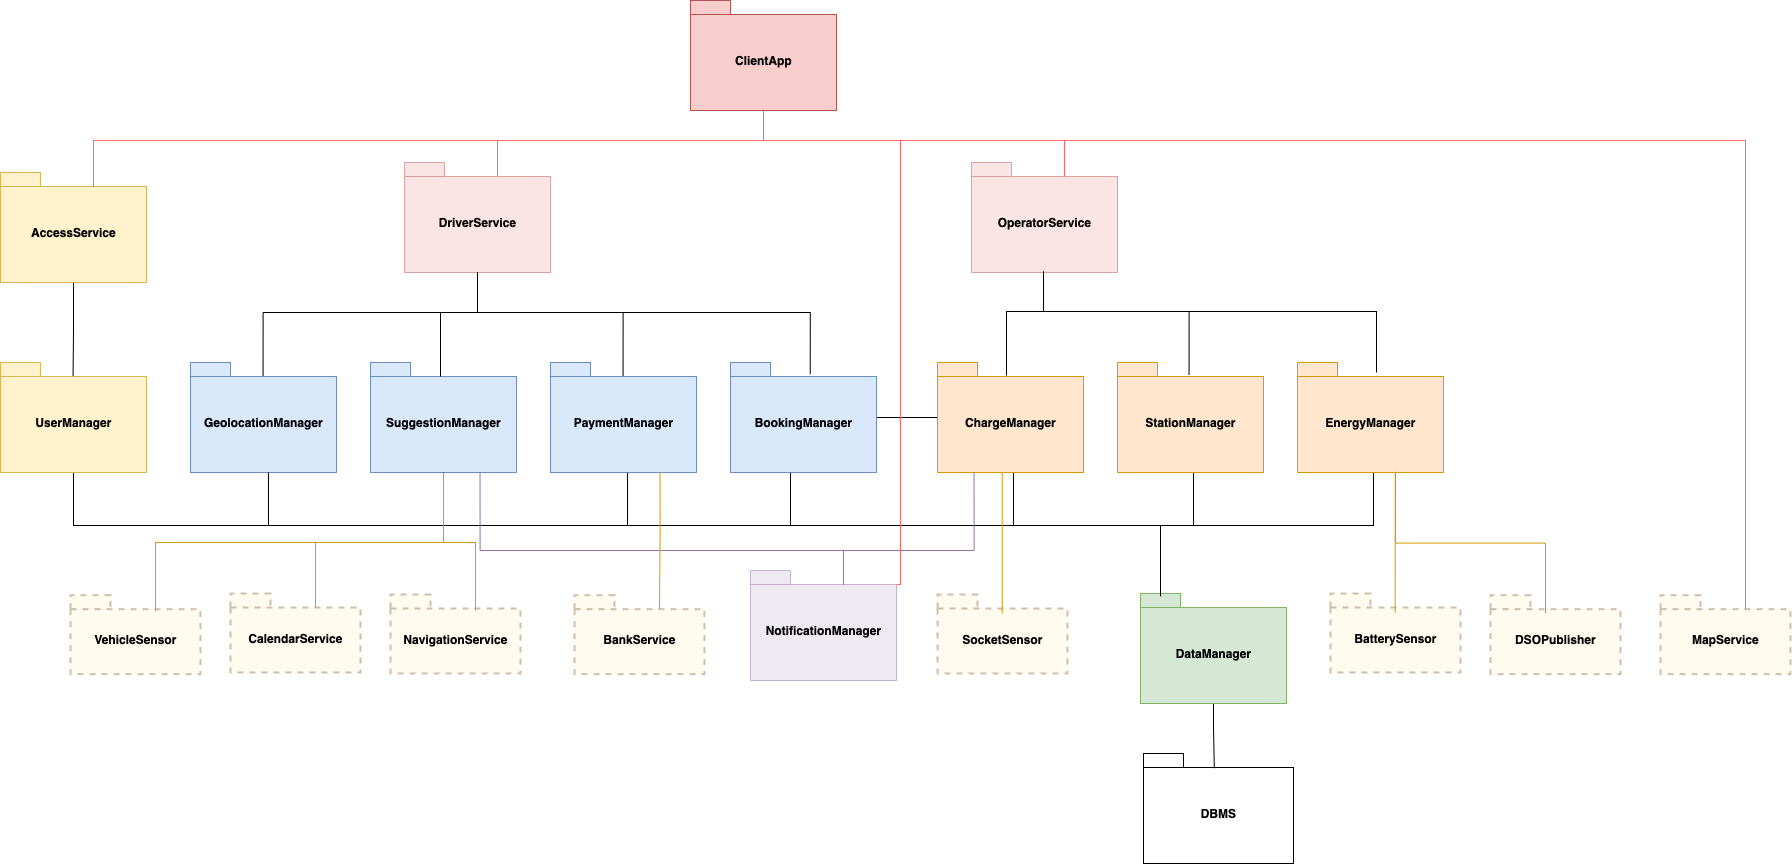
\includegraphics[width=1.05\textwidth]{ImplementationDiagram/6.png}
    \caption{Integration of all components with ClientApp}
    \label{fig:impdiag}
\end{figure}


\newpage
\subsection{System Testing}
\noindent
Once all system components have been integrated, it is time for System Testing. This process aims at verifying functional and non-functional requirements and must take place in a testing environment which is as close as possible to the production environment. Especially, the e-Mall System will be subject to the following tests:
\begin{itemize}
    \item Functional testing:\\
    verifying if all requirements written on RASD are satisfied and if there will be any possible missing functions. 
    \item Performance testing: \\
    necessary to check how the system is efficient in respect with response time, utilization, throughput by identifying bottlenecks. Establishing a performance baseline and compare between different versions of the same product or a different competitive product.
    \item Load testing: \\
    necessary to know how the system will perform under real-life loads. Useful for adjusting problems connected to memory such as memory leaks, mismanagement of memory, buffer overflows. 
    \item Stress testing: \\
    useful to know if the system can recover gracefully after failure.
\end{itemize}


\end{document}